\documentclass[10pt]{article}
\usepackage[letterpaper,hmargin=0.5in,vmargin=0.36in]{geometry}
\usepackage{longtable}
\usepackage{needspace}
\usepackage{tikz}
\usepackage{amsmath,amssymb,mathtools}
\usepackage{booktabs,array,colortbl}
\usepackage{xcolor}
\usepackage{pdfrender}
\usepackage[most]{tcolorbox}
\pagestyle{empty}
\setlength{\parindent}{0pt}
\definecolor{boxbg}{HTML}{F3F3F3}
\definecolor{boxfr}{HTML}{9A9A9A}
\definecolor{hdr}{HTML}{E4E4E4}
\newtcolorbox{sheetbox}{breakable,coltext=black,colback=boxbg,colframe=boxfr,boxrule=0.5pt,arc=2pt,left=6pt,right=6pt,top=2pt,bottom=2pt}
\newtcolorbox{smallbox}{breakable,fontupper=\small,coltext=black,colback=boxbg,colframe=boxfr,boxrule=0.5pt,arc=2pt,left=6pt,right=6pt,top=2pt,bottom=2pt}
\newcommand{\Cp}{\mathbb{C}}
\newcommand{\tr}{\operatorname{tr}}
\newcommand{\Mt}{M_2(\Cp)}
\newcommand{\eps}{\varepsilon}
\newcommand{\gh}{\hat g}
\newcommand{\rep}[1]{#1}
\newcommand{\forcesline}[1]{\par\vspace{-4pt}{\centering\small\textit{(#1)}\par}\vspace{2pt}}
\newcommand{\repline}[1]{\par\vspace{-2pt}{\leftskip=0.35in\rightskip=0.2in\noindent\textbf{Group class.} #1\par}\vspace{0pt}}
\newcommand{\lean}[1]{\texttt{\detokenize{#1}}}
\newcommand{\tg}[1]{{\scriptsize[#1]}}

\AtBeginDocument{\setlength{\abovedisplayskip}{2pt}\setlength{\belowdisplayskip}{2pt}\setlength{\abovedisplayshortskip}{2pt}\setlength{\belowdisplayshortskip}{3pt}}
\linespread{0.92}
\begin{document}
\color{black}\pdfrender{TextRenderingMode=FillStroke,LineWidth=0.22pt,StrokeColor=black,FillColor=black}
\vspace{0pt}
\begin{center}
{\Large\textbf{The Edge at $\boldsymbol{\alpha\to1^-}$}}\\[3pt]
{\large Or, Schr\"odinger Evolution from Feedback: A Canonicalization of Rotation, Dispersion, and Unitarity}\\[3pt]
\textit{Companion to Schr\"odinger evolution from the bare Causal Accumulation Law at $\alpha\to1^-$}
\end{center}
\vspace{1pt}
\begin{sheetbox}
\textbf{What this sheet is.} The edge paper in canonical form: one row per statement, the equation, what it forces, the symmetry that makes it so, and a bracketed tag naming the machine check. The Causal Accumulation Law is iterated as a transducer, each output becoming the next current. Nothing is added: no phase prefactor on the memory, no coupling constant, no time unit, and no field equation $T=0$.\par\vspace{3pt}
{\small\renewcommand{\arraystretch}{1.0}\setlength{\tabcolsep}{2.5pt}
\begin{minipage}[t]{0.505\linewidth}
\begin{tabular}[t]{@{}l l@{}}
\toprule
\textbf{Symbol} & \textbf{Meaning}\\
\midrule
$\alpha$,\ \ $\eps=1-\alpha$ & fractional order; distance to the edge\\
$n\in\mathbb Z$ & update count (the only clock)\\
$w_j$,\ \ $W(z)=\sum_{j\ge1}w_jz^{-j}$ & memory weights; their sum\\
$g$,\ \ $\gh(k)$,\ \ $\langle r^2\rangle$ & spatial profile, transform, width\\
$F(z)$ & characteristic function of the update\\
\bottomrule
\end{tabular}
\end{minipage}\hfill
\begin{minipage}[t]{0.47\linewidth}
\begin{tabular}[t]{@{}l l@{}}
\toprule
\textbf{Symbol} & \textbf{Meaning}\\
\midrule
$z=e^{i\varphi}$ & a mode $z^n$ of the update\\
${\rm Re}\,\varphi$,\ \ ${\rm Im}\,\varphi$ & rotation and decay per update\\
$t=\varphi_0n$ & time in radians of the rest rotation\\
$\hbar/2m=\langle r^2\rangle/12$ & kinetic coefficient, in rest radians\\
$b$,\ \ $\lambda$ & brake; fading rate of the past\\
\bottomrule
\end{tabular}
\end{minipage}}\par\vspace{3pt}
\textbf{Inputs.} The law; the free, flat sector, where the slot coupling and the transports are the identity, $\Pi P\Phi=1$; a power-law memory; the update rule; a past that has rotated one way. \textbf{Derived:} every row below. \textbf{Not claimed:} a mass in external units, interaction between carriers, Lorentz structure of the edge's dynamics, or a rigorous remainder for the rotation row.
\end{sheetbox}

\vspace{2pt}
\begin{sheetbox}
\textbf{Origin.} CAL is not a theory of quantum gravity. It is an information-physics engine for non-Markovian reality, built to lift self-attention to a field-theoretic form from first principles of cognition, causality and intelligence. Its derivations of known physics are unit tests: a law of causal memory that cannot recover established physics has no business modeling minds or societies. This sheet is one such test, at the edge $\alpha\to1^-$.\par\vspace{2pt}
\textbf{Definition 1 (Information).} Information $:=$ distinguishability of physical states.\quad \textbf{Definition 2 (Causality).} Causality $:=$ change in physical state, including its rate of change.\par\vspace{2pt}
\textbf{Axiom 1 (CAL).} The law displayed below; the kernel and the transports are real.\quad \textbf{Axiom 2 (the phase belongs to the source).} The channel angle $\theta=\alpha\pi/2$ is what an order-$\alpha$ accumulation does to the source's phase channel $e^{iS/\hbar}$; the real channel $e^{-H/\tau}$ is not turned, and no phase factor multiplies the memory.\quad \textbf{Axiom 3 (update rule).} Each output state becomes the next current, $J_{n+1}=T_n$.\quad \textbf{Axiom 4 (orientation).} The current's past has rotated one way, $J_n=c\,e^{i\varphi_hn}$ for $n<0$.\par\vspace{2pt}
{\footnotesize\textit{Definitions from On Information Physics: From State Distinguishability to Causal Accumulation, Sec.~1; axioms from the edge paper, Sec.~3.}}
\end{sheetbox}

\vspace{2pt}
{\large\textbf{The Causal Accumulation Law}} (On Information Physics, Eq.~61), \textbf{in the free, flat sector, mode by mode}
\[
T(x)=\alpha J(x)-(1-\alpha)\int_{J^-(x)}k(\tau;x,x')\,\Pi P\Phi\,J(x')\,d^4x'
\qquad\xrightarrow{\ \Pi P\Phi=1,\ \ e^{ik\cdot x}\ }\qquad
T_n=\alpha J_n-(1-\alpha)\,\gh(k)\sum_{j\ge1}w_jJ_{n-j}
\]
{\large\textbf{Carrier.}}\quad $J\in\Cp\otimes\mathbb H\cong\Mt$. The law acts on each Fourier mode and on each matrix entry of $J$ in the same way, so one scalar recurrence carries everything.

\vspace{3pt}\needspace{1.2in}
{\large\textbf{The transducer}}\quad $(0<\alpha<1,\ k=\tau^{\alpha-1}/\Gamma(\alpha),\ \Pi P\Phi=1)$\par
\[
J_{n+1}=T_n\qquad\Longrightarrow\qquad J_{n+1}=\alpha J_n-(1-\alpha)\,\gh(k)\sum_{j\ge1}w_jJ_{n-j}
\]
\forcesline{forces dynamics: the output is the next input, a feedback loop on the accumulated past}\repline{\rep{Linear, with coefficients that depend on neither $n$ nor $x$: it commutes with the shifts $(\mathbb Z,+)$ and the translations $(\mathbb R^3,+)$, so it is diagonal on their characters $z^ne^{ik\cdot x}$. The coefficients are real, so it commutes with complex conjugation and roots come in conjugate pairs. It acts entrywise on $J$, so it commutes with left and right multiplication by $GL(2,\Cp)$. \tg{sympy E: Lemma modes (1), (3), (4)}}}

\[
w_j=\frac{j^\alpha-(j-1)^\alpha}{\Gamma(\alpha+1)}=\int_{j-1}^{j}\frac{\tau^{\alpha-1}}{\Gamma(\alpha)}\,d\tau,\qquad \sum_{j\ge1}w_j=\infty,\qquad w_j\to1\ \ (\alpha\to1^-)
\]
\repline{\rep{Homogeneous of degree $\alpha-1$ under dilations of the lag: the memory has no scale, which is why no time unit is needed and time is quoted in rest radians. The total weight is infinite; as $\alpha\to1^-$ the weights flatten and the memory becomes the running sum of the past. \tg{Lean \lean{weight_tendsto_one}; sympy E: Def memory}}}

\[
\frac1{\Gamma(\alpha)}\int_0^\infty s^{\alpha-1}e^{i\omega s}\,ds=(-i\omega)^{-\alpha}=|\omega|^{-\alpha}e^{i\,{\rm sgn}(\omega)\,\alpha\pi/2}\qquad(0<\alpha<1,\ \omega\ne0)
\]
\par\vspace{2pt}\forcesline{forces the phase to the source: an order-$\alpha$ accumulation turns an oscillation by $\alpha$ quarter turns}\repline{\rep{The accumulation is a convolution on $(\mathbb R,+)$, so it acts on each character $e^{-i\omega t}$ by a number; that number has phase $\alpha\pi/2$, an element of $U(1)$. The integral converges exactly for $0<\alpha<1$: at $\alpha=1$ it oscillates without limit. \tg{mpmath A: Lemma weyl, to $10^{-45}$}}}

\[
W(e^{i\varphi})=\big(1-e^{-i\varphi}\big)\sum_{k\in\mathbb Z}\big(i(\varphi+2\pi k)\big)^{-\alpha-1},\qquad F(z)=z-\alpha+(1-\alpha)\,\gh\,W(z)
\]
\repline{\rep{Discrete time makes the frequency periodic: the sum runs over the dual lattice $2\pi\mathbb Z$ (Jonqui\`ere's formula, a Poisson summation). Principal powers; analytic off the rays $2\pi k+i[0,\infty)$; it continues $W$ across the unit circle. $z_0^n$ solves the update exactly when $F(z_0)=0$. \tg{mpmath A: Lemma W against direct sums, an accelerated series and \texttt{polylog}, to $10^{-44}$; Jonqui\`ere cited}}}

\[
\text{zero past, }J_0\ne0:\ \ \sum_{n\ge0}J_nz^{-n}=\frac{zJ_0}{F(z)};\qquad\text{one-way past adds }\ c\,e^{i\varphi_hn}\Big(W(e^{i\varphi_h})-\sum_{j=1}^{n}w_je^{-i\varphi_hj}\Big)\text{ to the memory}
\]
\repline{\rep{The $z$-transform is the Fourier transform on $(\mathbb Z,+)$: the solution is the sum of residues at the roots of $F$ plus a branch-cut contribution from $z=1$, where the infinite total weight puts a branch point. The whole infinite past enters through one known term, so it can be carried exactly. \tg{sympy E: Lemma modes (3), (4); numpy N: a pure mode with its exact past continues to $10^{-13}$}}}

\vspace{3pt}\needspace{1.2in}
{\large\textbf{Rotation}}\par
\[
w_j\equiv1:\qquad (z-1)F(z)=z^2-(1+\alpha)z+\alpha+(1-\alpha)\gh,\qquad \gh=1:\ \ z=e^{\pm i\varphi},\ \ \cos\varphi=\tfrac{1+\alpha}2
\]
\repline{\rep{At $k=0$ the two-step recurrence has companion matrix $\big(\begin{smallmatrix}1+\alpha&-1\\1&0\end{smallmatrix}\big)$, of determinant $1$ and trace $1+\alpha$: an element of $SL(2,\mathbb R)$, elliptic for $\alpha<1$ (roots on the unit circle), parabolic at $\alpha=1$ (double root $1$), hyperbolic for $\alpha>1$ (roots $e^{\pm s}$, $\cosh s=\tfrac{1+\alpha}2$). The angle is $\sqrt\eps\,(1+\eps/24+\dots)$. \tg{Lean \lean{flat_factor}, \lean{flat_lt}, \lean{flat_eq_one}, \lean{flat_gt}; sympy E: Lemma flat, G2}}}

\[
\varphi=\sqrt{\eps\gh}\,\big(1+O(\eps\ln\eps)\big)+i\Big[\tfrac12\eps(1-\gh)+\tfrac\pi4\eps^{3/2}\sqrt{\gh}\Big]+O(\eps^2\ln\eps)
\]
\forcesline{forces the $i$: negative feedback makes the current rotate by $\sqrt{1-\alpha}$ per update}\repline{\rep{With the power law the root leaves the circle $U(1)$ for the open disc: a contraction. The vanishing factor $1-\alpha$ multiplies an unbounded memory and leaves the finite rotation $\sqrt{1-\alpha}$. The leak $\tfrac\pi4\eps^{3/2}$ is the mismatch between $\alpha$ quarter turns and one. \tg{sympy E: expansion reproduced order by order; mpmath A: exact roots, $\pi/4$ to 34 digits, $\tfrac12$ exact; confirmed, not proved}}}

\[
{\rm Re}\,\varphi=\sqrt{\eps\gh}\Big[1+\eps\Big(\tfrac14\ln(\eps\gh)+\tfrac12-\tfrac{\gh}3-\tfrac1{8\gh}\Big)\Big],\qquad
{\rm Im}\,\varphi=\dots+\eps^2\Big[-\tfrac{\gh}4\ln(\eps\gh)+\tfrac{(1-\gh)(2-\gh)}4\Big]
\]
\repline{\rep{The logarithms make the edge a singular limit: it is not reached by a power series in $\eps$, and convergence is slow. At $\gh=1$ the exact decay exceeds the leading term by $13.6\%$ at $\eps=10^{-2}$ and $2.9\%$ at $10^{-4}$. \tg{sympy E: derived; mpmath A: measured independently, same coefficients}}}

\[
t=\varphi_0\,n,\qquad\frac{{\rm Re}\,\varphi(k)}{{\rm Re}\,\varphi(0)}=\sqrt{\gh(k)}\,\big(1+O(\eps\ln\eps)\big)
\]
\par\vspace{3pt}\forcesline{forces relational time: no unit, only ratios of rates}\repline{\rep{The memory is scale-covariant, so the law fixes no unit of time. The rest rotation is the only clock, and every rate is quoted against it: the quotient by dilations of time. The factor $\sqrt\eps$ cancels in the ratio, which is why the dispersion survives the limit while each rotation separately goes to zero. \tg{sympy E: Cor dispersion; mpmath A: exact roots}}}

\[
1-\sqrt{\gh(k)}=\frac{\langle r^2\rangle}{12}\,k^2+O(k^4)\qquad\Longrightarrow\qquad\frac{\hbar}{2m}=\frac{\langle r^2\rangle}{12}
\]
\forcesline{forces the kinetic term; the mass is the memory's spatial width}\repline{\rep{The profile is isotropic, so $\gh$ is invariant under $SO(3)$ and depends on $k$ only through $k^2$: the leading lag behind the rest rotation is quadratic, the Galilean dispersion. On the co-rotating branch the lag $e^{-i(\hbar/2m)k^2t}$ has the sign of a positive mass. Gaussian profile: the lag is $1-e^{-\langle r^2\rangle k^2/12}$. \tg{sympy E: Cor dispersion; mpmath A: Table mass}}}

\[
\exp\Big[-\big(i+\sqrt{1-\alpha}-\tfrac\pi4(1-\alpha)\big)\frac{\hbar}{2m}k^2t-\frac\pi4(1-\alpha)\,t\Big]\ \ \xrightarrow{\ \alpha\to1^-\ }\ \ e^{-i(\hbar/2m)k^2t}
\]
\forcesline{forces unitarity, in the limit only}\repline{\rep{Below the edge the evolution is a contraction semigroup, with a uniform loss $\tfrac\pi4(1-\alpha)$ per radian and a diffusive admixture of relative size $\sqrt{1-\alpha}$. At the edge it is the one-parameter unitary group generated by the Laplacian, the invariant of the Euclidean group. Rotation is the phase channel $e^{iS/\hbar}$, diffusion the real channel $e^{-H/\tau}$. \tg{sympy E: Thm unitary, G3, G4; mpmath A: Table diffusion}}}

\[
J_n=c\,e^{i\varphi_hn}\ \ (n<0)\qquad\Longrightarrow\qquad J_n=c\,e^{i\varphi n}\ \ \text{for all }n,\ \text{with no counter-rotating part (flat weights)}
\]
\forcesline{forces one orientation; the whole past is needed}\repline{\rep{The law commutes with conjugation, so $e^{\pm i\varphi n}$ are both modes; a one-way past breaks the symmetry and selects one, as the positive-frequency restriction does at $\alpha=2$. With the power law the counter-rotating amplitude is $10^{-7}$--$10^{-8}$ of the co-rotating one at $\eps=10^{-4}$; a zero past excites both equally, and so does a history of two cycles. \tg{sympy E: Lemma modes (4); numpy N: iteration}}}

\vspace{3pt}\needspace{0.9in}
{\large\textbf{Across the edge}}\par\vspace{2pt}
\begin{minipage}[c]{0.2\linewidth}\centering
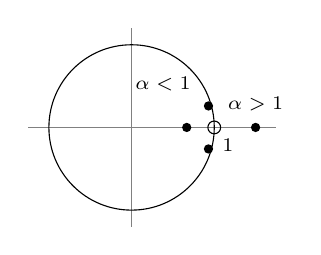
\begin{tikzpicture}[scale=1.05]
\draw[gray] (-1.25,0)--(1.75,0); \draw[gray] (0,-1.2)--(0,1.2);
\draw (0,0) circle (1);
\fill (0.93,0.26) circle (1.6pt); \fill (0.93,-0.26) circle (1.6pt);
\draw (1,0) circle (2.2pt);
\fill (1.5,0) circle (1.6pt); \fill (0.667,0) circle (1.6pt);
\node[font=\scriptsize] at (0.38,0.52) {$\alpha<1$};
\node[font=\scriptsize,anchor=south] at (1.5,0.08) {$\alpha>1$};
\node[font=\scriptsize,anchor=north west] at (0.98,-0.02) {$1$};
\end{tikzpicture}\par
{\scriptsize roots of $F$ in the $z$ plane}
\end{minipage}\hfill
\begin{minipage}[c]{0.78\linewidth}
{\small\renewcommand{\arraystretch}{1.05}\setlength{\tabcolsep}{4pt}
\begin{tabular}{@{}l l l l l@{}}
\toprule
 & \textbf{feedback} & \textbf{roots ($k=0$, flat)} & \textbf{$SL(2,\mathbb R)$ class} & \textbf{behaviour}\\
\midrule
$\alpha<1$ & negative, $-(1-\alpha)$ & $e^{\pm i\varphi}$, $\cos\varphi=\tfrac{1+\alpha}2$ & elliptic & rotation; unitary in the limit\\
$\alpha=1$ & none & double root $1$ & parabolic & the carrier is frozen\\
$\alpha>1$ & positive, $+(\alpha-1)$ & $e^{\pm s}$, $\cosh s=\tfrac{1+\alpha}2$ & hyperbolic & runaway, or bounded and advanced\\
\bottomrule
\end{tabular}}\par\vspace{2pt}
{\small As $\alpha$ rises through $1$ the conjugate pair slides along the circle to $z=1$, meets, and splits along the real axis. With the power law the pair sits just inside the circle, by $\tfrac\pi4\eps^{3/2}$.}
\end{minipage}\par\vspace{2pt}
\[
J_{n+1}=T_n+\delta_{n,n_0}:\qquad J_n=-\frac{1-e^{-s}}{2\sinh s}\,e^{-s(n_0-n)}\ \ (n\le n_0),\qquad J_n=+\frac{1-e^{-s}}{2\sinh s}\,e^{-s(n-n_0-1)}\ \ (n>n_0)
\]
\par\vspace{4pt}\forcesline{forces a choice above the edge: a causal runaway or a bounded preacceleration}\repline{\rep{The hyperbolic class has one growing and one decaying direction. A causal response must use the growing one, at about $\sqrt{\alpha-1}$ per update; the only bounded response uses the decaying one on each side of the source, so it is nonzero before the source acts and changes sign across it. These are the two horns of the Abraham--Lorentz--Dirac problem. At $\alpha=1$ the statement holds for any past whose memory sum converges. \tg{Lean \lean{feedback_frozen}, \lean{flat_gt}, \lean{green_homogeneous}, \lean{green_jump}; sympy G1}}}

\[
J_{n+1}=(1-b)\,T_n,\quad w_j\to w_je^{-\lambda j}:\qquad\text{settles}\iff(1-b)\big(\alpha+(\alpha-1)W_\lambda(1)\big)<1
\]
\repline{\rep{The root crosses $z=1$ exactly when the criterion fails, by the intermediate value theorem on the real axis. If the past never fades, $W(1)=\infty$ and no brake settles the growth: integral windup. At $\alpha=1.01$ the thresholds are $b>0.097$ ($\lambda=0.1$) and $b>0.513$ ($\lambda=0.01$). \tg{mpmath A: necessary and sufficient on 480 grid points and 30 root counts}}}

\[
w_j\ge0,\ \ \sum_jw_j=1,\ \ 0<\alpha<1,\ \ 0\le\gh\le1\qquad\Longrightarrow\qquad F(z)\ne0\ \text{ for all }|z|\ge1
\]
\par\vspace{3pt}\forcesline{forces the power law: a normalizable memory damps every mode}\repline{\rep{$W$ maps the closed exterior of the unit disc into the closed unit disc, so $|(1-\alpha)\gh W|\le1-\alpha\le|z-\alpha|$, with equality only at $z=1$, where $F(1)=(1-\alpha)(1+\gh)\ne0$. This covers every exponential kernel and the Dirac kernel. The power law escapes because its total weight is infinite. $\alpha>0$ is needed: at $\alpha=0$ the Dirac kernel has the root $z=i$. \tg{Lean \lean{normalizable}, \lean{norm_memory_le_one}, \lean{F_one}, \lean{alpha_zero_root}; sympy E: 4075 exact rational kernels, no counterexample}}}

\[
\frac{\tau^{\alpha-1}}{\Gamma(\alpha)}=\int_0^\infty e^{-s\tau}\mu_\alpha(s)\,ds,\qquad\mu_\alpha(s)=\frac{\sin\pi\alpha}{\pi}\,s^{-\alpha},\qquad\frac{\mu_\alpha[0,\delta]}{\mu_\alpha[0,S]}=\Big(\frac\delta S\Big)^{1-\alpha}\to1
\]
\par\vspace{4pt}\forcesline{forces Markov structure at the edge without extra state}\repline{\rep{The decaying exponentials $e^{-s\tau}$ are the characters of the semigroup $(\mathbb R_{\ge0},+)$; below the edge a Markov description needs a continuum of them. As $\alpha\to1^-$ the weight concentrates on the trivial character $s=0$: the single mode $\int^tJ$, the accumulator of the fundamental theorem of calculus. \tg{sympy E: Prop accumulator; Lean \lean{weight_tendsto_one}}}}

\[
\text{forgetful (Dirac): }w_j=\delta_{j1}\qquad\big|\qquad\text{edge: }w_j\to1,\ \ \textstyle\sum_{j\ge1}J_{n-j}\qquad\big|\qquad\text{faithful (light cone): each term kept}
\]
\repline{\rep{The framework has two Markov limits, and the edge is neither. The forgetful limit keeps nothing of the past and, being normalizable, damps every mode at about $2(1-\alpha)$ per update. The faithful limit keeps every contribution and cannot be reached by a closed system. The edge keeps the sum and not each term, so it needs neither records nor extra state. \tg{Lean \lean{normalizable} for the Dirac kernel; mpmath A: Table normalizable; the faithful limit is cited from On Information Physics}}}

\vspace{3pt}\needspace{1.2in}
{\large\textbf{Readout at the edge}}\quad(the closure $JJ^\dagger$ is an $\alpha=2$ object, read here from one carrier)\par
\[
JJ^\dagger={\rm Tr}_{\rm right}\,|J\rangle\!\rangle\langle\!\langle J|=x^0\,1+\vec x\cdot\vec\sigma,\qquad \tr JJ^\dagger=p_++p_-,\qquad\det JJ^\dagger=|\det J|^2=p_+p_-\,(\tr JJ^\dagger)^2
\]
\repline{\rep{$J$ is a vector in $\Cp^2\otimes\Cp^2$: rows are the factor on which $SL(2,\Cp)$ acts, columns the factor on which the internal phase acts. Born by trace and Lorentz by determinant are the sum and the product of the Schmidt weights of one carrier. \tg{Lean \lean{det_closure}, \lean{lorentz_invariant_density}; sympy E: Prop carrier (1)--(3)}}}

\[
C=\frac{2|\det J|}{\tr JJ^\dagger}=\sqrt{1-v^2/c^2}=\frac1\gamma=\operatorname{sech}\eta,\qquad p_\pm=\frac{e^{\pm\eta}}{2\cosh\eta}
\]
\par\vspace{4pt}\forcesline{forces the reading: the entanglement of a carrier's two factors is the time dilation of its current}\repline{\rep{Rotations, $SU(2)$, are local unitaries and leave the concurrence $C$ fixed; boosts, the Hermitian positive elements of $SL(2,\Cp)$, are local filterings and change it. The Schmidt weights are the Doppler factors $e^{\pm\eta}$, and collinear boosts add rapidities. A carrier at rest is maximally entangled; a null closure is a product. \tg{Lean \lean{conc_sq}, \lean{conc_eq_sqrt}, \lean{conc_sech}, \lean{schmidt_weights}; sympy E: Prop carrier (4), Prop lorentz (1), (3)}}}

\[
J\mapsto GJ,\ \ G\in SL(2,\Cp):\qquad Q\mapsto GQG^\dagger,\qquad|\det J|\ \text{fixed},\qquad x^0=\tfrac12\tr Q\ \text{not};\qquad\{\det Q=0\}/\mathbb R_{>0}\cong\Cp P^1
\]
\repline{\rep{The invariant density is $|\det J|$; the density in a frame is the trace, and it changes under boosts. The null closures, the pure states of the left factor, form the celestial sphere $\Cp P^1$, on which $SL(2,\Cp)$ acts by M\"obius transformations. The Lorentz group here acts on the carrier's closure, not on the spacetime of the edge. \tg{Lean \lean{lorentz_invariant_density}; the M\"obius action is cited, Penrose and Rindler}}}

\[
2J=JJ^\dagger\ \Longrightarrow\ J^\dagger=J,\ \ J^2=2J,\ \ \tr\tfrac J2={\rm rank}\,J;\qquad\text{rank one}\iff\Lambda^2J=0
\]
\repline{\rep{The closure normalizes itself only at rank one. In $\Mt$ that is $\det J=0$; in $M_N(\Cp)$, $N\ge3$, the determinant is not enough: ${\rm diag}(2,2,0)$ has $\det=0$ and $\tr\tfrac J2=2$. The condition is the vanishing of the second exterior power, the $GL(N)$-invariant statement of rank one. \tg{Lean \lean{self_normalized}, \lean{minors_example}; sympy E: Lemma minors}}}

\[
p_m=\frac{\tr(P_mJJ^\dagger)}{\tr JJ^\dagger},\quad\sum_mP_m=1;\qquad(J_A\otimes J_B)(J_A\otimes J_B)^\dagger=J_AJ_A^\dagger\otimes J_BJ_B^\dagger
\]
\par\vspace{4pt}\forcesline{forces the readout to survive composition}\repline{\rep{The readout is a probability distribution for $J\in M_N(\Cp)$ of any rank. Product carriers give product statistics, and marginals are consistent for every $J_{AB}$, by the partial trace. Rank and entanglement differ: $J_{AB}=\Phi^+\eta^\dagger$ with $\eta$ a unit vector has rank one and ${\rm Tr}_BQ_{AB}=\tfrac12$. \tg{sympy E: Prop composition (1)--(3); numpy N: Table readout, nine rows}}}

\[
\text{one-way past:}\quad\frac{d}{dt}\ln\tr Q=-2\Big[\tfrac\pi4(1-\alpha)+\big(\sqrt{1-\alpha}-\tfrac\pi4(1-\alpha)\big)\frac{\hbar}{2m}\langle k^2\rangle\Big]\ \to\ 0,\qquad Q=\sum_kJJ^\dagger
\]
\forcesline{forces one orientation for the Born readout}\repline{\rep{With a one-way past the closure and the readout become conserved as $\alpha\to1^-$. With a zero past both rotation directions are present; their cross terms oscillate at twice the rotation, $\tr Q$ swings by a factor of order one, and the readout drift does not vanish. \tg{numpy N: Table closure; one random carrier in the paper, the same scaling over eight}}}

\vspace{3pt}\needspace{1.0in}
{\large\textbf{Structure of the edge}}\par
\[
\text{two carriers:}\quad\text{the update is a sum of single-carrier terms}\qquad\Longrightarrow\qquad\text{no entanglement between }A\text{ and }B\text{ is created}
\]
\forcesline{forces a free edge: no interaction, no holonomy from the carrier}\repline{\rep{The past enters through transports from a past point to the present, each within one carrier, so the update is a sum of single-carrier terms: it can carry entanglement between carriers but not create it. At fixed modes the Schmidt coefficients are unchanged. A coupling needs the return leg, the adjoint transport $P_\gamma^\dagger=P_{\gamma^{-1}}$, and a leg with its return is order $1+1=2$, the closure. Below the closure there is no determinant, hence no signature and no light cone: the causal structure is time ordering alone, the Galilean structure of the Schr\"odinger equation, whose propagator reaches every distance for $t>0$. \tg{reading; not machine-checked}}}

\vspace{2pt}
\begin{smallbox}
\textbf{What the numbers say.} Exact roots of $F$ and direct iteration, with code independent of the paper's script.\par\vspace{2pt}
\begin{minipage}[t]{0.47\linewidth}
\renewcommand{\arraystretch}{1.0}\setlength{\tabcolsep}{4pt}
\begin{tabular}[t]{@{}c c c@{}}
\toprule
$1-\alpha$ & rotation $\div\sqrt{1-\alpha}$ & decay per radian $\div(1-\alpha)$\\
\midrule
$10^{-2}$ & $0.989722$ & $0.90146$\\
$10^{-4}$ & $0.999775$ & $0.80843$\\
$10^{-7}$ & $1.000000$ & $0.78667$\\
$\to0$ & $1$ & $\pi/4=0.78540$\\
\bottomrule
\end{tabular}
\end{minipage}\hfill
\begin{minipage}[t]{0.5\linewidth}
\renewcommand{\arraystretch}{1.0}\setlength{\tabcolsep}{4pt}
\begin{tabular}[t]{@{}c c c c@{}}
\toprule
$1-\alpha$ & $\lVert\text{CAL}-\text{Schr}\rVert$, rescaled & floor ($k^4$) & norm lost\\
\midrule
$10^{-2}$ & $0.070$ & $0.011$ & $61.8\%$\\
$10^{-3}$ & $0.026$ & $0.012$ & $10.1\%$\\
$10^{-4}$ & $0.015$ & $0.013$ & $1.52\%$\\
\bottomrule
\end{tabular}
\end{minipage}\par\vspace{2pt}
{\renewcommand{\arraystretch}{1.0}\setlength{\tabcolsep}{4pt}
\begin{tabular}[t]{@{}l c c c c c@{}}
\toprule
$(\langle r^2\rangle,\ k)$ at $1-\alpha=10^{-5}$ & $(0.06,\,0.10)$ & $(0.60,\,0.10)$ & $(0.60,\,0.20)$ & $(6.00,\,0.05)$ & $(6.00,\,0.20)$\\
\midrule
measured $\big(\varphi(0)-\varphi(k)\big)/\big(\varphi(0)k^2\big)$ & $0.005000$ & $0.049988$ & $0.049950$ & $0.499688$ & $0.495034$\\
$\langle r^2\rangle/12$ & $0.005000$ & $0.050000$ & $0.050000$ & $0.500000$ & $0.500000$\\
\bottomrule
\end{tabular}\hfill
\begin{tabular}[t]{@{}l c c@{}}
\toprule
growth per update, no brake & $\alpha=1.01$ & $\alpha=1.001$\\
\midrule
measured & $0.1010$ & $0.03167$\\
$\sqrt{\alpha-1}$ & $0.1000$ & $0.03162$\\
\bottomrule
\end{tabular}}\par\vspace{2pt}
Top left: $k=0$; the gap to $\pi/4$ is $-\tfrac14\sqrt\eps\ln\eps$. Bottom: the mass row, with departures that are the $k^4$ terms, and the runaway above the edge. Top right: the packet $e^{-x^2/2+ix}$ with $\langle r^2\rangle=0.06$, evolved to $(\hbar/2m)t=0.5$ with the exact one-way past, compared with free Schr\"odinger evolution after aligning the phase and rescaling to unit norm. The shape converges in every row; the amplitude converges only near the edge. No root with $|z|\ge1$ exists for $0<\alpha<1$, and inside the circle only the conjugate pair (argument principle, 54 cases). \tg{mpmath A; numpy N}
\end{smallbox}

\vspace{1pt}
\begin{smallbox}
\textbf{Remark (the wave is the accumulated past).} The wave at a point is the carrier's accumulated causal past evaluated there, not a spread in space at one instant. Accumulation with real weights gives diffusion, the channel $e^{-H/\tau}$, as in Feynman--Kac; accumulation with phase gives waves, the channel $e^{iS/\hbar}$, as in the path integral. The edge law is a mixture of the two, dominated by the phase, and the mixture is what the exponent $-(i+\sqrt{1-\alpha})$ records. Feynman's $\psi(x,t)$ is likewise a sum over the past parts of paths ending at $(x,t)$: a parallel, not a derivation.\par\vspace{1pt}
\textbf{Remark (relation to $\alpha=2$).} At $\alpha=2$ the update rule is not the dynamics. There the balance reading applies: the present equals the light-cone accumulated past, which gives the Klein--Gordon equation and the path sum; exactly at $2$ that law is conservative, and above it runs away. The edge at $1$ and the closure at $2$ are the two places where the law is marginal: unitary here, conservative there.
\end{smallbox}

\vspace{1pt}
\begin{smallbox}
\textbf{What the checks changed.} The edge paper's results stand; these statements were corrected, and this sheet uses the corrected forms. (1) The bounded response above the edge: the earlier $e^{-s|n-n_0|}/(2\sinh s)$ had the wrong sign and answered a source held on, not an impulse; the impulse response is the two-sided form above. (2) The packet comparison rescales the state to unit norm; the norm lost is now tabulated. (3) A two-cycle history excites the counter-rotating mode at $0.68$--$0.97$ of the co-rotating amplitude, not $70$--$97\%$ of the norm. (4) The brake thresholds $0.095$ and $0.501$ were for flat weights; the simulated weights give $0.097$ and $0.513$. (5) The long-wavelength exponent keeps $-\tfrac\pi4(1-\alpha)$. (6) Two rows of the normalizable-kernel table depended on cutting the kernel at $400$ lags; the exponential of width $100$ has largest root $0.99008$, and the summable power law $j^{-1.5}$ decays algebraically. (7) At $\alpha=1$ the memory sum of a non-decaying past diverges; the frozen carrier is stated for convergent sums. (8) $F(1)=(1-\alpha)(1+\gh)$. (9) The readout drift varies tenfold across random carriers. (10) Double-precision agreement of the memory sum is $5\times10^{-15}$. \textbf{Remark (a measurable departure).} If the order sits slightly below $1$, the uniform loss $\tfrac\pi4(1-\alpha)$ per radian of rest rotation and the diffusion of relative size $\sqrt{1-\alpha}$ are universal, so precision interference and clock comparisons would bound $1-\alpha$. \textbf{Forward pointer.} The mass comes from the kernel width and the rest rotation from the feedback rate; nothing here ties them. A width of $\sqrt6$ Compton wavelengths would, and belongs to the $\alpha=2$ program.
\end{smallbox}

\vspace{1pt}
\begin{smallbox}
\textbf{Legend.} $T$ and $J$ are both rank-one currents, so $J_{n+1}=T_n$ is type-consistent.\quad \textbf{Update rule:} the edge's dynamics. It is not used at $\alpha=2$, where the term $2J$ alone would double the current; there the balance reading applies.\quad \textbf{Relational time:} no unit; rates are ratios of rates.\quad \textbf{One-way past:} $J_n=c\,e^{i\varphi_hn}$ for $n<0$, the orientation as a property of the source, not a factor in the law.\quad \textbf{Loss:} the decay below the edge is a phase effect of the fractional order, not erasure; erasure is the contraction from rank $2$ to rank $1$, in interaction and readout.\quad \textbf{Group class notes} name the symmetry behind each row; where a note has no tag of its own it is a reading.
\end{smallbox}

\vspace{1pt}
{\large\textbf{The necessity chain}}\hfill{\footnotesize\textit{each element is forced by a modeling requirement}}\par\vspace{2pt}
{\small\renewcommand{\arraystretch}{1.0}\setlength{\tabcolsep}{3pt}\setlength{\aboverulesep}{1pt}\setlength{\belowrulesep}{1.5pt}
\begin{longtable}{@{}>{\raggedright\arraybackslash}p{1.75in}>{\raggedright\arraybackslash}p{2.25in}>{\raggedright\arraybackslash}p{1.5in}>{\raggedright\arraybackslash}p{1.75in}@{}}
\rowcolor{hdr}\textbf{Requirement} & \textbf{Structure / Element} & \textbf{Control analogy} & \textbf{Role}\\
\midrule\endfirsthead
\rowcolor{hdr}\textbf{Requirement} & \textbf{Structure / Element} & \textbf{Control analogy} & \textbf{Role}\\
\midrule\endhead
The state must evolve & $J_{n+1}=T_n$\ \ (update rule) & Closed loop & The output is fed back as the next input\\
\multicolumn{4}{@{}>{\raggedright\arraybackslash}p{7.5in}@{}}{\hspace{0.25in}\textbf{Group class.} Shift-invariant linear recurrence: diagonal on the characters $z^n$ of $(\mathbb Z,+)$ \tg{sympy E}}\\
\midrule
The past must pull back & $-(1-\alpha)$, $0<\alpha<1$ & Negative feedback & Restoring force; rotation in place of growth\\
\multicolumn{4}{@{}>{\raggedright\arraybackslash}p{7.5in}@{}}{\hspace{0.25in}\textbf{Group class.} Elliptic class in $SL(2,\mathbb R)$ at $k=0$; the sign flips at $\alpha=1$ \tg{Lean \lean{flat_lt}; sympy G2}}\\
\midrule
History must not fade to nothing & $w_j$\ \ (power law, infinite total weight) & Integrator & The only memory with an undamped mode in the limit\\
\multicolumn{4}{@{}>{\raggedright\arraybackslash}p{7.5in}@{}}{\hspace{0.25in}\textbf{Group class.} Scale-covariant under dilations of the lag; every normalizable kernel damps every mode \tg{Lean \lean{normalizable}}}\\
\midrule
No external clock & $t=\varphi_0n$\ \ (rest radians) & Normalized frequency & Rates are ratios of rates\\
\multicolumn{4}{@{}>{\raggedright\arraybackslash}p{7.5in}@{}}{\hspace{0.25in}\textbf{Group class.} Quotient by dilations of time: only the ratio $\varphi(k)/\varphi(0)$ is read \tg{reading}}\\
\midrule
Space must enter & $\gh(k)$, $\langle r^2\rangle$\ \ (spatial profile) & Loop gain per mode & Sets the mass: $\hbar/2m=\langle r^2\rangle/12$\\
\multicolumn{4}{@{}>{\raggedright\arraybackslash}p{7.5in}@{}}{\hspace{0.25in}\textbf{Group class.} $SO(3)$-invariant function of $k^2$ on the dual of the translations \tg{sympy E; mpmath A}}\\
\midrule
A direction of time & one-way past $c\,e^{i\varphi_hn}$ & Initial condition over the whole history & Selects one of the conjugate pair\\
\multicolumn{4}{@{}>{\raggedright\arraybackslash}p{7.5in}@{}}{\hspace{0.25in}\textbf{Group class.} Breaks the conjugation symmetry $\mathbb Z_2$ of the real law \tg{numpy N}}\\
\midrule
Growth must settle above the edge & $b$, $\lambda$\ \ (brake and fading) & Anti-windup & Braking alone cannot settle an unfading integrator\\
\multicolumn{4}{@{}>{\raggedright\arraybackslash}p{7.5in}@{}}{\hspace{0.25in}\textbf{Group class.} Hyperbolic class; the root crosses $z=1$ at the criterion \tg{mpmath A}}\\
\midrule
The phase must come from the law's own order & $(-i\omega)^{-\alpha}$\ \ (Weyl symbol) & Phase lag of a fractional integrator & $\alpha$ quarter turns; no prefactor is added\\
\multicolumn{4}{@{}>{\raggedright\arraybackslash}p{7.5in}@{}}{\hspace{0.25in}\textbf{Group class.} Multiplier on the characters of $(\mathbb R,+)$, with phase in $U(1)$ \tg{mpmath A}}\\
\midrule
The edge must close on itself & $\sum_{j\ge1}J_{n-j}$\ \ (running sum) & Pure integrator & Markov with no added state\\
\multicolumn{4}{@{}>{\raggedright\arraybackslash}p{7.5in}@{}}{\hspace{0.25in}\textbf{Group class.} The trivial character $s=0$ of the semigroup $(\mathbb R_{\ge0},+)$ \tg{sympy E; Lean \lean{weight_tendsto_one}}}\\
\midrule
Carriers must stay free & single legs, $\Pi P\Phi=1$ & Open loop between carriers & No interaction until the return leg, order $2$\\
\multicolumn{4}{@{}>{\raggedright\arraybackslash}p{7.5in}@{}}{\hspace{0.25in}\textbf{Group class.} Local operations: no entanglement between carriers is created \tg{reading}}\\
\midrule
The state must be read & $JJ^\dagger$\ \ (closure) & Output map & Born by trace, Lorentz by determinant\\
\multicolumn{4}{@{}>{\raggedright\arraybackslash}p{7.5in}@{}}{\hspace{0.25in}\textbf{Group class.} Right $U(2)$-invariant, left $GL(2,\Cp)$-covariant; concurrence invariant under $SU(2)$ \tg{Lean \lean{conc_sech}}}\\
\midrule
\end{longtable}}

\vspace{2pt}
{\footnotesize
\emergencystretch=3em \textbf{Machine verification.} Four independent checks of the edge paper, none reusing its script. \textbf{Lean} 4.35.0 with Mathlib v4.35.0, file \texttt{SchrodingerEdge.lean}: 28 theorems, no \texttt{sorry}, axioms only \texttt{propext}, \texttt{Classical.choice}, \texttt{Quot.sound}. \textbf{sympy E}: 70 exact checks of the algebra, labelled by the paper's statement; \textbf{G1--G4}: the corrected impulse response, the $SL(2,\mathbb R)$ class and the unitarity exponents. \textbf{mpmath A}: exact roots and special functions at 40 digits or more. \textbf{numpy N}: direct iteration, then the paper's script run unchanged, which reproduces its tables. The checks corrected the edge paper in ten places, listed above; this sheet states the corrected forms.
\textbf{Not machine-checked:} a rigorous remainder for the rotation row (the expansion is formal, reproduced symbolically and matched by exact roots); Jonqui\`ere's formula as a theorem (cited; verified numerically); the Weyl integral in Lean; Prop lorentz (2) and (4); the structure-of-the-edge row and the loss statement of the Legend, the control analogies, and the group class notes without a tag, which are readings.\par}
\end{document}
